\documentclass{book}
\usepackage[landscape,a3paper,left=0.5cm,right=1in,top=1in,bottom=1in]{geometry}
\usepackage{amsmath}
\usepackage{xcolor}
\usepackage{tikz}
\usepackage{pgfplots}
\usepackage{booktabs}
\usepackage{multirow}
\usepackage{amsmath,amssymb}

\begin{document}

\vspace{2cm}

\begin{center}\underline{\textsc{Equiv + Permut} for Test of 98 small instances of polynomial}
\vspace{0.5cm}

\begin{tabular}{cc} & no-solver\\\\\tikz{\node (a) at (0.0,4) {\textsc{Algo}};\node (a) at (0.0,0) {};} & 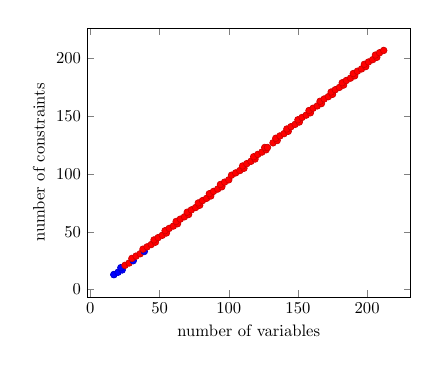
\begin{tikzpicture}[scale=0.6]
\begin{axis}[scatter, point meta=\thisrow{time}, only marks, colorbar, colorbar horizontal,colorbar style={ylabel={Time (min)}, ylabel style={rotate=270},}, colorbar to name={storedcolorbar1},, xlabel=number of variables,ylabel=number of constraints]

\addplot table[x=x,y=y]  { 
 x y time
 17 13 0.05 
 17 13 0.0 
 20 15 0.0 
 23 17 0.0 
 22 19 5.0 
 25 21 1440.0 
 28 23 1440.0 
 31 25 4.0 
 30 27 1440.0 
 33 29 1440.0 
 36 31 1440.0 
 39 33 13.0 
 38 35 1440.0 
 41 37 1440.0 
 44 39 1440.0 
 47 41 1440.0 
 46 43 1440.0 
 49 45 1440.0 
 52 47 1440.0 
 55 49 1440.0 
 54 51 1440.0 
 57 53 1440.0 
 60 55 1440.0 
 63 57 1440.0 
 62 59 1440.0 
 65 61 1440.0 
 68 63 1440.0 
 71 65 1440.0 
 70 67 1440.0 
 73 69 1440.0 
 76 71 1440.0 
 79 73 1440.0 
 78 75 1440.0 
 81 77 1440.0 
 84 79 1440.0 
 87 81 1440.0 
 86 83 1440.0 
 89 85 1440.0 
 92 87 1440.0 
 95 89 1440.0 
 94 91 1440.0 
 97 93 1440.0 
 100 95 1440.0 
 102 99 1440.0 
 105 101 1440.0 
 108 103 1440.0 
 111 105 1440.0 
 110 107 1440.0 
 113 109 1440.0 
 116 111 1440.0 
 119 113 1440.0 
 118 115 1440.0 
 121 117 1440.0 
 124 119 1440.0 
 127 121 1440.0 
 126 123 1440.0 
 128 123 1440.0 
 132 127 1440.0 
 135 129 1440.0 
 134 131 1440.0 
 137 133 1440.0 
 140 135 1440.0 
 143 137 1440.0 
 142 139 1440.0 
 145 141 1440.0 
 148 143 1440.0 
 151 145 1440.0 
 150 147 1440.0 
 153 149 1440.0 
 156 151 1440.0 
 159 153 1440.0 
 158 155 1440.0 
 161 157 1440.0 
 164 159 1440.0 
 167 161 1440.0 
 166 163 1440.0 
 169 165 1440.0 
 172 167 1440.0 
 175 169 1440.0 
 174 171 1440.0 
 177 173 1440.0 
 180 175 1440.0 
 183 177 1440.0 
 182 179 1440.0 
 185 181 1440.0 
 188 183 1440.0 
 191 185 1440.0 
 190 187 1440.0 
 193 189 1440.0 
 196 191 1440.0 
 199 193 1440.0 
 198 195 1440.0 
 201 197 1440.0 
 204 199 1440.0 
 207 201 1440.0 
 206 203 1440.0 
 209 205 1440.0 
 212 207 1440.0 
};

\end{axis}
\end{tikzpicture}

\\
\tikz{\node (a) at (0.0,4) {\textsc{AlgoEnhanced}};\node (a) at (0.0,0) {};} & 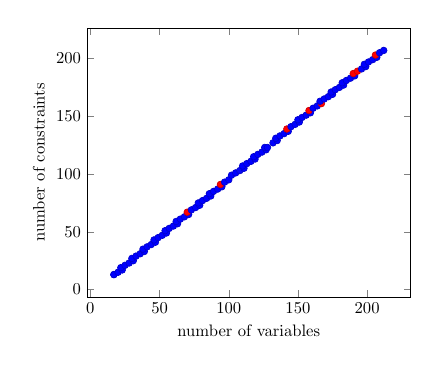
\begin{tikzpicture}[scale=0.6]
\begin{axis}[scatter, point meta=\thisrow{time}, only marks, , xlabel=number of variables,ylabel=number of constraints]

\addplot table[x=x,y=y]  { 
 x y time
 17 13 0.05 
 17 13 0.0 
 20 15 0.0 
 23 17 0.0 
 22 19 0.0 
 25 21 0.0 
 28 23 0.0 
 31 25 0.0 
 30 27 0.0 
 33 29 0.0 
 36 31 0.0 
 39 33 0.0 
 38 35 0.0 
 41 37 0.0 
 44 39 0.0 
 47 41 0.0 
 46 43 0.0 
 49 45 0.0 
 52 47 0.0 
 55 49 0.0 
 54 51 0.0 
 57 53 0.0 
 60 55 0.0 
 63 57 0.0 
 62 59 0.0 
 65 61 0.0 
 68 63 0.0 
 71 65 0.0 
 70 67 1440.0 
 73 69 0.0 
 76 71 0.0 
 79 73 0.0 
 78 75 0.0 
 81 77 0.0 
 84 79 0.0 
 87 81 0.0 
 86 83 0.0 
 89 85 0.0 
 92 87 0.0 
 95 89 0.0 
 94 91 1440.0 
 97 93 0.0 
 100 95 0.0 
 102 99 0.0 
 105 101 0.0 
 108 103 16.0 
 111 105 0.0 
 110 107 0.0 
 113 109 0.0 
 116 111 0.0 
 119 113 0.0 
 118 115 0.0 
 121 117 0.0 
 124 119 0.0 
 127 121 0.0 
 126 123 0.0 
 128 123 0.0 
 132 127 0.0 
 135 129 0.0 
 134 131 0.0 
 137 133 0.0 
 140 135 0.0 
 143 137 0.0 
 142 139 1440.0 
 145 141 0.0 
 148 143 0.0 
 151 145 0.0 
 150 147 0.0 
 153 149 0.0 
 156 151 0.0 
 159 153 0.0 
 158 155 1440.0 
 161 157 0.0 
 164 159 0.0 
 167 161 1440.0 
 166 163 0.0 
 169 165 0.0 
 172 167 0.0 
 175 169 0.0 
 174 171 0.0 
 177 173 0.0 
 180 175 0.0 
 183 177 0.0 
 182 179 0.0 
 185 181 0.0 
 188 183 0.0 
 191 185 0.0 
 190 187 1440.0 
 193 189 1440.0 
 196 191 0.0 
 199 193 0.0 
 198 195 0.0 
 201 197 0.0 
 204 199 0.0 
 207 201 0.0 
 206 203 1440.0 
 209 205 0.0 
 212 207 0.0 
};

\end{axis}
\end{tikzpicture}

\\
\\\\
\multicolumn{2}{c}{\ref{storedcolorbar1}}\end{tabular}\end{center}

\newpage

\begin{center}\underline{\textsc{Non-Equiv + Permut} for Test of 98 small instances of polynomial}
\vspace{0.5cm}

\begin{tabular}{cc} & no-solver\\\\\tikz{\node (a) at (0.0,4) {\textsc{Algo}};\node (a) at (0.0,0) {};} & 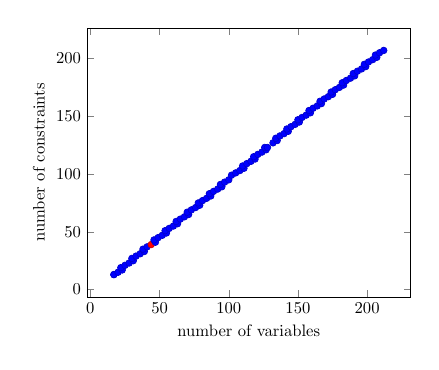
\begin{tikzpicture}[scale=0.6]
\begin{axis}[scatter, point meta=\thisrow{time}, only marks, colorbar, colorbar horizontal,colorbar style={ylabel={Time (min)}, ylabel style={rotate=270},}, colorbar to name={storedcolorbar2},, xlabel=number of variables,ylabel=number of constraints]

\addplot table[x=x,y=y]  { 
 x y time
 17 13 0.05 
 17 13 0.0 
 20 15 0.0 
 23 17 0.0 
 22 19 0.0 
 25 21 0.0 
 28 23 0.0 
 31 25 0.0 
 30 27 0.0 
 33 29 0.0 
 36 31 0.0 
 39 33 0.0 
 38 35 0.0 
 41 37 0.0 
 44 39 1440.0 
 47 41 0.0 
 46 43 0.0 
 49 45 0.0 
 52 47 0.0 
 55 49 0.0 
 54 51 0.0 
 57 53 0.0 
 60 55 0.0 
 63 57 0.0 
 62 59 0.0 
 65 61 0.0 
 68 63 0.0 
 71 65 0.0 
 70 67 0.0 
 73 69 0.0 
 76 71 0.0 
 79 73 0.0 
 78 75 0.0 
 81 77 0.0 
 84 79 0.0 
 87 81 0.0 
 86 83 0.0 
 89 85 0.0 
 92 87 0.0 
 95 89 0.0 
 94 91 0.0 
 97 93 0.0 
 100 95 0.0 
 102 99 0.0 
 105 101 0.0 
 108 103 0.0 
 111 105 0.0 
 110 107 0.0 
 113 109 0.0 
 116 111 0.0 
 119 113 0.0 
 118 115 0.0 
 121 117 0.0 
 124 119 0.0 
 127 121 0.0 
 126 123 0.0 
 128 123 0.0 
 132 127 0.0 
 135 129 0.0 
 134 131 0.0 
 137 133 0.0 
 140 135 0.0 
 143 137 0.0 
 142 139 0.0 
 145 141 0.0 
 148 143 0.0 
 151 145 0.0 
 150 147 0.0 
 153 149 0.0 
 156 151 0.0 
 159 153 0.0 
 158 155 0.0 
 161 157 0.0 
 164 159 0.0 
 167 161 0.0 
 166 163 0.0 
 169 165 0.0 
 172 167 0.0 
 175 169 0.0 
 174 171 0.0 
 177 173 0.0 
 180 175 0.0 
 183 177 0.0 
 182 179 0.0 
 185 181 0.0 
 188 183 0.0 
 191 185 0.0 
 190 187 0.0 
 193 189 0.0 
 196 191 0.0 
 199 193 0.0 
 198 195 0.0 
 201 197 0.0 
 204 199 0.0 
 207 201 0.0 
 206 203 0.0 
 209 205 0.0 
 212 207 0.0 
};

\end{axis}
\end{tikzpicture}

\\
\tikz{\node (a) at (0.0,4) {\textsc{AlgoEnhanced}};\node (a) at (0.0,0) {};} & 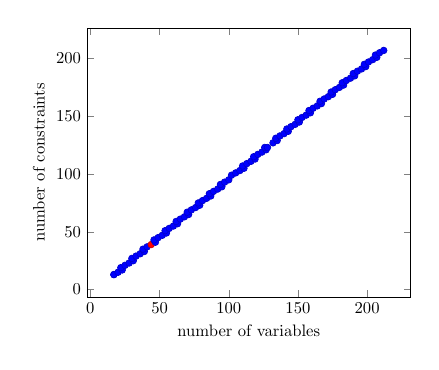
\begin{tikzpicture}[scale=0.6]
\begin{axis}[scatter, point meta=\thisrow{time}, only marks, , xlabel=number of variables,ylabel=number of constraints]

\addplot table[x=x,y=y]  { 
 x y time
 17 13 0.05 
 17 13 0.0 
 20 15 0.0 
 23 17 0.0 
 22 19 0.0 
 25 21 0.0 
 28 23 0.0 
 31 25 0.0 
 30 27 0.0 
 33 29 0.0 
 36 31 0.0 
 39 33 0.0 
 38 35 0.0 
 41 37 0.0 
 44 39 1440.0 
 47 41 0.0 
 46 43 0.0 
 49 45 0.0 
 52 47 0.0 
 55 49 0.0 
 54 51 0.0 
 57 53 0.0 
 60 55 0.0 
 63 57 0.0 
 62 59 0.0 
 65 61 0.0 
 68 63 0.0 
 71 65 0.0 
 70 67 0.0 
 73 69 0.0 
 76 71 0.0 
 79 73 0.0 
 78 75 0.0 
 81 77 0.0 
 84 79 0.0 
 87 81 0.0 
 86 83 0.0 
 89 85 0.0 
 92 87 0.0 
 95 89 0.0 
 94 91 0.0 
 97 93 0.0 
 100 95 0.0 
 102 99 0.0 
 105 101 0.0 
 108 103 0.0 
 111 105 0.0 
 110 107 0.0 
 113 109 0.0 
 116 111 0.0 
 119 113 0.0 
 118 115 0.0 
 121 117 0.0 
 124 119 0.0 
 127 121 0.0 
 126 123 0.0 
 128 123 0.0 
 132 127 0.0 
 135 129 0.0 
 134 131 0.0 
 137 133 0.0 
 140 135 0.0 
 143 137 0.0 
 142 139 0.0 
 145 141 0.0 
 148 143 0.0 
 151 145 0.0 
 150 147 0.0 
 153 149 0.0 
 156 151 0.0 
 159 153 0.0 
 158 155 0.0 
 161 157 0.0 
 164 159 0.0 
 167 161 0.0 
 166 163 0.0 
 169 165 0.0 
 172 167 0.0 
 175 169 0.0 
 174 171 0.0 
 177 173 0.0 
 180 175 0.0 
 183 177 0.0 
 182 179 0.0 
 185 181 0.0 
 188 183 0.0 
 191 185 0.0 
 190 187 0.0 
 193 189 0.0 
 196 191 0.0 
 199 193 0.0 
 198 195 0.0 
 201 197 0.0 
 204 199 0.0 
 207 201 0.0 
 206 203 0.0 
 209 205 0.0 
 212 207 0.0 
};

\end{axis}
\end{tikzpicture}

\\
\\\\
\multicolumn{2}{c}{\ref{storedcolorbar2}}\end{tabular}\end{center}

\newpage

\end{document}